\documentclass[../rapport_MVEX01-11-05]{subfiles}
\begin{document}
\section{Kvantitativa mått på handens geometri}\label{sec:features}

För att på något sätt kunna kvantifiera den data en bild av en hand 
innehåller och tolka den på ett bra sätt måste denna data transformeras till
något meningsfullt. Det finns många sätt att göra detta --- man kan exempelvis
beräkna bildens egenvärden \cite{Funck02}, använda filter för att hitta
fingertoppar \cite{Noelker97}, eller jämföra bilden med lagrade prototypbilder
och sedan studera det s.k.~Hausdorff-avståndet till dessa \cite{Nielsen04}.
En enklare metod
är att beräkna ett antal olika egenskaper baserade på den binära bilden
och använda dessa för klassificering.

Dessa egenskaper kan bestå av mått med enkla definitioner baserade på area,
omkrets, mittpunkt eller rotation hos objektet i den binära bilden och kan
därför användas av en klassificerare för att skilja mellan olika rörelseoberoende
gester. Eftersom egenskaperna inte innehåller information om rörelse kan denna
uppsättning egenskaper inte användas direkt i tillämpningar som involverar
rörelsegester, utan måste kompletteras av exempelvis hastighets- eller
riktningsegenskaper.

\subsection{Egenskapsrummet}

Egenskapsrummet är ett $\R^n$-rum där varje dimension representerar en
egenskap. I detta rum kan man beräkna ''avstånd'' mellan olika gester,
eller mellan en observerad gest och tidigare träningsdata. Egenskaperna baseras som sagt
på olika grundläggande mått hos den binära bilden, och ett antal användbara
egenskaper presenteras nedan.
Många av egenskaperna som beskrivs kan beräknas effektivt av
\MATLAB-funktionen \texttt{regionprops}.

\paragraph{Inledande definitioner}

För beräkning av vissa egenskaper behöver man definiera två
grundläggande begrepp; den inneslutande lådan och centroiden. Dessa
två kan användas för att i någon mening hitta ''mitten'' av objektet
vi undersöker. Den inneslutande lådan kan dessutom användas för vissa
jämförelser relaterade till area (dvs. densitetsliknande begrepp).

\subparagraph{Inneslutande låda}

Den inneslutande lådan är den minsta axelparallella rektangeln som innehåller hela
objektet (se figur \ref{fig:boundingbox}),
och kan effektivt beräknas genom att lokalisera
extrempunkterna i $x$- och $y$-led. Lådan har fyra mått: bredd, höjd samt
position i $x$- och $y$-led. Utifrån dessa kan vi även beräkna
mittpunkten i $x$- och $y$-led.

\subparagraph{Centroid}

Centroiden är masscentrum för ett område, och beräknas enligt
\begin{equation*}
  \textrm{centroid}(A) = \frac{
    \sum\limits_{a\in A}m_a\vect{r}_a
  }{
    \sum\limits_{a\in A}m_a
  } =
  \sum\limits_{a\in
  A}\frac{\vect{r}_a}{\textrm{Area}(A)},
\end{equation*}
där man använder att $m_a=1,\:\forall a\in A$ eftersom bilden är
binär ($m_a$ är helt enkelt intensiteten i punkten $a$ och
$\vect{r}_a$ är positionen av punkten $a$). Centroiden är vektorvärd.

Man kan dessutom definiera ett relativt centroidläge  som avståndet mellan 
centroiden och lådans övre/vänstra kant genom lådans bredd/höjd.

\paragraph{Hu-moment}

Dessa moment definierades först av \citeasnoun{Hu62} och är ett försök att
göra centralmomenten $u_{pq}$ rotations-, skalnings- och translationsinvarianta och
därmed mer användbara. 

Centralmomenten $\mu_{pq}$ definieras av
\begin{equation*}
	\mu_{pq} = \sum\limits_x\sum\limits_y
	           \left(x-\bar{x}\right)^p
	           \left(y-\bar{y}\right)^q
	           f(x,y)
\end{equation*}
där $\bar{x}$ och $\bar{y}$ är centroidens x- och y-komponent, och $f(x,y)$ är
bildens ljusstyrka. För binära bilder gäller att
$f:\left\{\text{Bildpunkter}\right\}\rightarrow\left\{0,1\right\}$.

De sju Hu-moment definieras utifrån centralmomenten \cite[s.~185]{Hu62}:
\begin{align*}
	I_1 =& \;\mu_{20} + \mu_{02}\\
	I_2 =& \left(\mu_{20} - \mu_{02}\right)^2 + 4\mu^2_{11}\\
	I_3 =& \left(\mu_{30} - 3\mu_{12}\right)^2 +
	       \left(3\mu_{21} - \mu_{03}\right)^2\\
	I_4 =& \left(\mu_{30} + \mu{12}\right)^2 +
 	       \left(\mu_{21} + \mu_{03}\right)^2\\
	I_5 =& \left(\mu_{30} - 3\mu_{12}\right)
	       \left(\mu_{30} + \mu_{12}\right)
	       \left(\left(\mu_{30}+\mu{12}\right)^2 -
	       3\left(\mu{21}+\mu{03}\right)^2\right) + \\
 	    &+ \left(3\mu_{21} - \mu_{03}\right)\left(\mu_{21} + \mu_{03}\right)
	       \left(3\left(\mu_{30} + \mu{12}\right)^2 -
	       \left(\mu_{21} + \mu_{03}\right)^2\right)\\
	I_6 =& \left(\mu_{20}-\mu_{02}\right)
	       \left(\left(\mu_{30}+\mu_{12}\right)^2 -
	       \left(\mu_{21}+\mu_{03}\right)^2\right) + \\
	    &+ 4\mu_{11}\left(\mu_{30}+\mu_{12}\right)
	       \left(\mu_{21}+\mu_{03}\right)\\
	I_7 =& \left(3\mu_{21}-\mu_{03}\right)\left(\mu_{30}-\mu_{12}\right)
	       \left(\left(\mu_{30}+\mu_{12}\right)^2 - 
	       3\left(\mu_{21}+\mu_{03}\right)^2\right) - \\
	    &- \left(\mu_{30} - 3\mu_{12}\right)\left(\mu_{21}+\mu_{03}\right)
	       \left(3\left(\mu_{30}+\mu_{12}\right)^2 - 
  	     \left(\mu_{21}+\mu_{03}\right)^2\right)
\end{align*}



\paragraph{Konvexitet}

Konvexitet \cite[s.~26]{Rudemo09} är ett dimensionslöst
mått som beskriver hur konvext ett objekt är --- för
gestigenkänning är detta ett relevant mått på huruvida fingrarna är
utsträckta eller inte, men även på om de sitter tätt ihop (ex.
stopptecken) eller löst konfigurerade (ex. segertecken). Det
definieras av
\begin{equation*}
  \textrm{konvexitet}(A) = \frac{\left|\partial A_h\right|}{\left|\partial A\right|}
\end{equation*}
där $A_h$ är det konvexa höljet till $A$ (dvs. det minsta konvexa område som
helt täcker $A$) och $\partial A$ betecknar randen till $A$ (i diskret
mening). Detta innebär i princip att $\left|\partial A\right|$
betecknar omkretsen av $A$.

\paragraph{Kompakthet}

Kompakthet \cite[s.~26]{Rudemo09} är ännu ett dimensionslöst mått, som
beskriver hur kompakt ett objekt är.
Cirkeln är det mest kompakta objektet, och ju fler irregulariteter
randen innehåller (jämfört med en cirkel) desto mindre blir kompaktheten.
Kompakthet definieras av
\begin{equation*}
  \textrm{kompakthet}(A) = \frac{\textrm{Area}(A)}{\left|\partial
  A\right|^2}.
\end{equation*}

\paragraph{Soliditet}

Soliditet är ett mått på hur poröst ett objekt är. Det
definieras av kvoten mellan objektets area och det konvexa skalets
area enligt
\begin{equation*}
  \textrm{soliditet}(A) = \frac{\textrm{Area}(A)}{\textrm{Area}(A_h)},
\end{equation*}
och är därför dimensionslöst. Detta mått kan vara mycket hjälpsamt för
gester som t.ex.~''OK'' (en ring formad av tumme och pekfinger, med
övriga fingrar riktade uppåt).

\paragraph{Fyrkantighet}

Den här egenskapen är helt enkelt ett mått på hur kvadratisk den axelparallella
inneslutande lådan är, och på så sätt mäter den hur ''utsträckt'' en
gest är. Dess definition är mycket enkel:
\begin{equation*}
  \textrm{fyrkantighet}(A) = \frac{\textrm{Box}_w(A)}{\textrm{Box}_h(A)}.
\end{equation*}

En perfekt kvadratisk låda har alltså fyrkantighet $1$, och ju mer
fyrkantigheten avviker från detta värde desto mer avlång är gesten.
Notera att excentriciteten (se nedan) mäter i princip samma sak men utgår från
andramomenten och därmed är oberoende av objektets vinkel.

\paragraph{Excentricitet}

Excentriciteten är ett mått på hur utsträckt ett objekt är (precis som
fyrkantigheten), men utgår från den ellips
vars andramoment är samma som
objektets (se figur~\ref{fig:ellips}). Excenticiteten definieras av avståndet
mellan andramomenten i ellipsen genom längden av den längsta axeln. Därmed
beror måttet, till skillnad från fyrkantigheten, inte på objektets orientering.

\begin{figure}[tb]
	\centering 
	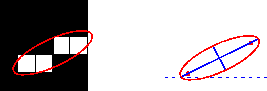
\includegraphics{bilder/matlab-ellips.png}
	\caption{En ellips vars andramoment (röda prickar till höger) är samma
	som objektets}
	\label{fig:ellips}
\end{figure}

\paragraph{Utsträckning}

Utsträckningen mäter hur stor del av den inneslutande lådan som
faktiskt täcks av vårt objekt. Egenskapen kan ses som ett alternativ
till konvexiteten och definieras enligt
\begin{equation*}
  \textrm{utsträckning}(A) =
  \frac{\textrm{Area}(A)}{\textrm{Area}(\textrm{Box}(A))}.
\end{equation*}

\subsection{Normering och viktning för klassificering}

Eftersom många klassificeringsmetoder använder det euklidiska avståndet mellan punkter i 
egenskapsrummet är det viktigt att egenskaperna som används varierar över
ungefär samma värdemängd. Så är inte är fallet från början och därför måste indata
normeras.

Man kan exempelvis skala all indata så att den anpassas till en 
$\N(0,1)$-distribution (efter att ha sett till att egenskaperna kan tänkas 
vara normalfördelade, t.ex.~genom att logaritmera de kvotbaserade 
egenskaperna) genom att beräkna uppskattningar $\hat\mu$ och $\hat\sigma$
utifrån prototyp- eller träningsdata (man får självfallet en uppsättning sådana
parametrar per egenskap i egenskapsrummet). Denna metod kommer inte
att göra icke normalfördelade egenskaper normalfördelade, men alla
egenskapers varians kommer likställas \cite{Aksoy01}.

Man kan därefter använda dessa parametrar för att normalisera ny indata, så
att även den passar in i det nya egenskapsrummet:
\begin{equation*}
	\hat{x} = \frac{x - \hat\mu_x}{\hat\sigma_x}
\end{equation*}

Vill man därefter optimera klassificeraren och se till att den tar större hänsyn
till vissa gester kan man även införa en viktningskonstant $w_x$ --- en stor
sådan gör att egenskapen har större betydelse (eftersom avståndet då ökar
snabbare). Denna konstant appliceras lämpligen direkt efter normeringen.

\end{document} 

